\documentclass[
	12pt,
	a4paper,
	bibtotoc,
	cleardoubleempty, 
	idxtotoc,
	ngerman,
	openright
	final,
	listof=nochaptergap,
	]{scrbook}

\usepackage[T1]{fontenc}
\usepackage[utf8]{inputenc}

% ##################################################
% Unterstuetzung fuer die deutsche Sprache
% ##################################################
\usepackage{ngerman}
\usepackage[ngerman]{babel}

% ##################################################
% Dokumentvariablen
% ##################################################
\newcommand{\docOrt}{Furtwangen}
\newcommand{\docTitle}{Access Point und Router mit embedded Board Banana Pi R1}
\newcommand{\docUntertitle}{}
\newcommand{\docArtDerArbeit}{Projektarbeit}
\newcommand{\docFakultaet}{Informatik}
\newcommand{\docReferent}{}
\newcommand{\docAbgabedatum}{??.??.2017}

% ##################################################
% Allgemeine Pakete
% ##################################################

% Abbildungen einbinden
\usepackage{graphicx}

% Zusaetsliche Sonderzeichen
\usepackage{dingbat}

% Farben
\usepackage{color}
\usepackage[usenames,dvipsnames,svgnames,table]{xcolor}

% Maskierung von URLs und Dateipfaden
\usepackage[hyphens]{url}

% Deutsche Anfuehrungszeichen
\usepackage[babel, german=quotes]{csquotes}

% Pakte zur Index-Erstellung (Schlagwortverzeichnis)
\usepackage{index}
\makeindex

% Ipsum Lorem
% Paket wird nur für das Beispiel gebraucht und kann gelöscht werden
\usepackage{lipsum}

% ##################################################
% Seitenformatierung
% ##################################################
\usepackage[
	portrait,
	bindingoffset=1.5cm,
	inner=2.5cm,
	outer=2.5cm,
	top=3cm,
	bottom=2cm,
	%includeheadfoot
	]{geometry}

% ##################################################
% Kopf- und Fusszeile
% ##################################################

\usepackage{fancyhdr}

\pagestyle{fancy}
\fancyhf{}
\fancyhead[EL,OR]{\sffamily\thepage}
\fancyhead[ER,OL]{\sffamily\leftmark}

\fancypagestyle{headings}{}

\fancypagestyle{plain}{}

\fancypagestyle{empty}{
  \fancyhf{}
  \renewcommand{\headrulewidth}{0pt}
}

%Kein "Kapitel # NAME" in der Kopfzeile
\renewcommand{\chaptermark}[1]{
	\markboth{#1}{}
   	\markboth{\thechapter.\ #1}{}
}

% ##################################################
% Schriften
% ##################################################

% Stdandardschrift festlegen
\renewcommand{\familydefault}{\sfdefault}

% Standard Zeilenabstand: 1,5 zeilig
\usepackage{setspace}
\onehalfspacing 

% Schriftgroessen festlegen
\addtokomafont{chapter}{\sffamily\large\bfseries} 
\addtokomafont{section}{\sffamily\normalsize\bfseries} 
\addtokomafont{subsection}{\sffamily\normalsize\mdseries} 
\addtokomafont{subsubsection}{\sffamily\normalsize\mdseries} 
\addtokomafont{caption}{\sffamily\normalsize\mdseries} 

% ##################################################
% Inhaltsverzeichnis / Allgemeine Verzeichniseinstellungen
% ##################################################

\usepackage{tocloft}

% Punkte auch bei Kapiteln
\renewcommand{\cftchapdotsep}{3}
\renewcommand{\cftdotsep}{3}

% Schriftart und -groesse im Inhaltsverzeichnis anpassen
\renewcommand{\cftchapfont}{\sffamily\normalsize}
\renewcommand{\cftsecfont}{\sffamily\normalsize}
\renewcommand{\cftsubsecfont}{\sffamily\normalsize}
\renewcommand{\cftchappagefont}{\sffamily\normalsize}
\renewcommand{\cftsecpagefont}{\sffamily\normalsize}
\renewcommand{\cftsubsecpagefont}{\sffamily\normalsize}

%Zeilenabstand in den Verzeichnissen einstellen
\setlength{\cftparskip}{.5\baselineskip}
\setlength{\cftbeforechapskip}{.1\baselineskip}

% ##################################################
% Abbildungsverzeichnis und Abbildungen
% ##################################################

\usepackage{caption}

\usepackage{wrapfig}

% Nummerierung von Abbildungen
\renewcommand{\thefigure}{\arabic{figure}}
\usepackage{chngcntr}
\counterwithout{figure}{chapter}

% Abbildungsverzeichnis anpassen
\renewcommand{\cftfigpresnum}{Abbildung }
\renewcommand{\cftfigaftersnum}{:}

% Breite des Nummerierungsbereiches [Abbildung 1:]
\newlength{\figureLength}
\settowidth{\figureLength}{\bfseries\cftfigpresnum\cftfigaftersnum}
\setlength{\cftfignumwidth}{\figureLength}
\setlength{\cftfigindent}{0cm}

% Schriftart anpassen
\renewcommand\cftfigfont{\sffamily}
\renewcommand\cftfigpagefont{\sffamily}

% ##################################################
% Tabellenverzeichnis und Tabellen
% ##################################################

% Nummerierung von Tabellen
\renewcommand{\thetable}{\arabic{table}}
\counterwithout{table}{chapter}

% Tabellenverzeichnis anpassen
\renewcommand{\cfttabpresnum}{Tabelle }
\renewcommand{\cfttabaftersnum}{:}

% Breite des Nummerierungsbereiches [Abbildung 1:]
\newlength{\tableLength}
\settowidth{\tableLength}{\bfseries\cfttabpresnum\cfttabaftersnum}
\setlength{\cfttabnumwidth}{\tableLength}
\setlength{\cfttabindent}{0cm}

%Schriftart anpassen
\renewcommand\cfttabfont{\sffamily}
\renewcommand\cfttabpagefont{\sffamily}

% Unterdrueckung von vertikalen Linien
\usepackage{booktabs}

% ##################################################
% Listings (Quellcode)
% ##################################################

\usepackage{listings}
\lstset{
	language=java,
	backgroundcolor=\color{white},
	breaklines=true,
	prebreak={\carriagereturn},
 	breakautoindent=true,
 	numbers=left,
 	numberstyle=\tiny,
 	stepnumber=2,
 	numbersep=5pt,
 	keywordstyle=\color{blue},
   	commentstyle=\color{green},   
   	stringstyle=\color{gray}
}
  	
% ##################################################
% Theoreme
% ##################################################
  	
% Umgebung fuer Beispiele
\newtheorem{beispiel}{Beispiel}

% Umgebung fuer These
\newtheorem{these}{These}

% Umgebung fuer Definitionen
\newtheorem{definition}{Definition}
  	
% ##################################################
% Literaturverzeichnis
% ##################################################

\usepackage{bibgerm}

% ##################################################
% Abkuerzungsverzeichnis
% ##################################################

\usepackage[printonlyused]{acronym}

% ##################################################
% PDF / Dokumenteninternelinks
% ##################################################

\usepackage[
   	linkcolor=black,
   	citecolor=black,
  	filecolor=black,
	urlcolor=black,
    bookmarks=true,
    bookmarksopen=true,
    bookmarksopenlevel=3,
    bookmarksnumbered,
    plainpages=false,
    pdfpagelabels=true,
    hyperfootnotes,
    pdftitle ={\docTitle}]{hyperref}


\begin{document}

\setcounter{secnumdepth}{3}

% Titelblatt
\begin{titlepage}
\pagestyle{empty}

% ##################################################
% HFU-Logo einbinden
% ##################################################
\begin{flushright}
\begin{figure}[ht]
\flushright

\includegraphics[height=3cm]{pictures/hfu.jpg}
\end{figure}
\end{flushright}

% ##################################################
% Titel
% ##################################################
\begin{center}
{\fontsize{18}{22} \selectfont \docArtDerArbeit}\\[5mm]
{\fontsize{18}{22} \selectfont in der Fakult\"at} \\[5mm]
{\fontsize{18}{22} \selectfont \docFakultaet}\\
\vspace{1cm}
\begin{onehalfspace}
{\fontsize{22}{26} \selectfont \textbf{\docTitle}}\\[5mm]
{\fontsize{18}{22} \selectfont \docUntertitle}


\end{onehalfspace}
\end{center}

% ##################################################
% Zusatzinformationen
% ##################################################
\vfill
\begin{center}
\begin{tabular}{lcl}
Referent	&:& Dr. Jiri Spale	\\ \\
Vorgelegt am 	&:& \docAbgabedatum 	\\ \\
Vorgelegt von 	&:& Bastian	\\
		& & Elias	\\
		& & Jakob	\\
		& & Jonas	\\
		& & Tom
\end{tabular}
\end{center}
\end{titlepage}

\cleardoubleemptypage

\frontmatter


% Abstract
\chapter*{Abstract\markboth{Abstract}{}}
\addcontentsline{toc}{chapter}{Abstract}

The project „Access Point und Router mit embedded Board Banana Pi R1“ is a continuation of a previous project done at the university in Furtwangen of the same name from the winter semester 2016/2017. Its main goals were to find a suitable operating system for the BananaPi and recording the network traffic. There were future objectives listed at the end of the documentation which have been worked upon in this semester. The main goals for this project are to further analyse and test applicable operating systems as well as implementing different functions such as Radius, Samba, Mailserver, display status readout and a backup solution.
\\\\\\
Bei dem Projekt „Access Point und Router mit embedded Board Banana Pi R1“, handelt es sich um die Weiterführung des bereits im Wintersemester 2016/2017 an der Hochschule Furtwangen abgehaltenen Projekts mit demselben Name. Das damalige Vorhaben bestand daraus, ein passendes Betriebssystem für den BananaPi zu ermitteln und den Netzwerkverkehr aufzuzeichnen. Am Ende wurden zukünftige Ziele aufgelistet welche in diesem Semester erarbeiten wurden. Projektziele sind, das Analysieren und Testen passender Betriebssysteme, sowie die Implementierung verschiedener Funktionen wie Radius, Samba, einem Mailserver, einer Displaystatusanzeige und einer Backup Lösung.

\cleardoubleemptypage

% Inhaltsverzeichnis
\tableofcontents
\addcontentsline{toc}{chapter}{Inhaltsverzeichnis}
\cleardoubleemptypage

% Abbildungsverzeichnis einbinden und ins Inhaltsverzeichnis
% WORKAROUND: tocloft und KOMA funktionieren zusammen nicht
% korrekt\phantomsection
\addcontentsline{toc}{chapter}{\listfigurename} 
\listoffigures
\cleardoubleemptypage

% Tabellenverzeichnis einbinden und ins Inhaltsverzeichnis
% WORKAROUND: tocloft und KOMA funktionieren zusammen nicht
% korrekt\phantomsection
%\phantomsection
%\addcontentsline{toc}{chapter}{\listtablename}
%\listoftables
%\cleardoubleemptypage

% Abkürzungsverzeichnis
\chapter*{Abkürzungsverzeichnis\markboth{Abkürzungsverzeichnis}{}}
\addcontentsline{toc}{chapter}{Abkürzungsverzeichnis}

\begin{acronym}
\acro{HFU}{Hochschule Furtwangen University}
\acro{PSW}{Pumpspeicherwerk}
\end{acronym}

\mainmatter

\chapter{Projektübersicht}

\section{Kontext}
Das Projekt mit dem Titel Router mit embedded Board Banana Pi R1 wird als Se-
mesterprojekt im Sommersemester 2017 an der Hochschule Furtwangen durch-
geführt. Das Projekt wurde von Dr. Jiri Spale ins Leben gerufen und wird
intern, ohne die Kooperation mit einem Unternehmen durchgeführt. Die Anzahl der studentischen Projektteilnehmer beträgt fünf.

\section{Ziel}
Das primäre Ziel des Projektes ist es, das bestehende Router-Projekt weiterzuentwickeln. Folgende Funktionalitäten sollen implementiert werden:\\
~\\
\begin{itemize}
\item Implementierung eines RADIUS-Servers zur zentralen Authentifizierung von Anwendern
\item Implementierung einse Voucher-Systems
\item Installation des Betriebssystems IP Fire
\item Mehrere WLAN Access Points auf einem WLAN-Chip
\item Mail-Server zum Statusbericht der Backups
\item SAMBA/NFS Server
\item Automatische Aktuatisierung von Programmpaketen des Systems
\item Implementierung einer Display-Statusanzeige
\end{itemize}
~\\
Die Funktionen sollen auf dem Betriebssystem “Bananian”, ein auf das Banana Pi zugeschnittenes Debian, implementiert werden.

\chapter{Betriebssystemübersicht}

Zu Begin des Projektes standen die beiden Betriebssysteme OpenWRT und Bananian zur Verfügung.
Außerdem gab es den Vorschlag des VorgängerProjekts, zusätzlich das Projekt auch mit dem Betribssystem IPFire durchzuführen.
Die Nutzung der einzelnen Betriebssysteme fiel sehr unterschiedlich aus, da die implementierten Funkionen und der Stand der Entwicklung sich stark von System zu System unterschied.

\section{OpenWRT}
OpenWRT ist ein Betriebssystem, das für eingebettete Geräte wie Wlan Router enwickelt wurde.
Das System wird übe ein Webinterface angepasst und unterscheidet sich stark zu den anderen im Projekt verwendeten Betriebssystemen.
Durch diese Unterschiede wurden nur enzelne Teile des Projektes auf OpenWRT umgesetzt.

\section{IPFire}
\begin{wrapfigure}{r}{5cm}
\centering

\includegraphics[width=3.5cm]{pictures/Jakob/IPFire}
\caption{IPFire Logo}
Quelle: \cite{fire1}
\end{wrapfigure}
Das Betriebssystem IPFire ist darauf ausgelegt, als Router genutzt zu werden, wobei das Augenmerk auf der implementierung einer Firewall oder eines VPN Gateways liegt.
Das vorgehende Projekt hatte dieses Betriebssystem als Alternative vorgeschlagen, weshalb wir dieses System als Aternative untersucht haben. Zwei Abbilder für den Betrieb auf Arm Prozessoren stehen auf der Webseite des Betriebssystems bereit. \cite{fire} \\
Bei beide Abbildern stellte sich allerdings herraus, dass die HDMI Schnittstelle nicht unterschtützt wird.
Auch eine Verbindung SSH nicht möglich ist, da IPFire auf eine Konfiguration über das Webinterface ausgelegt ist.
Eines der beiden Abbilder ist auf die Konfiguration über eine Serielle Schnittstelle Ausgelegt. Da uns aber für diese Schnittstelle keine Wekzeuge und Adapter bereitstehen, haben wir auch von dieser Option abgelassen.\\

\newpage
\section{Bananian}
\begin{wrapfigure}{r}{5cm}
\centering

\includegraphics[width=3cm]{pictures/Jakob/Bananian}
\caption{Bananian Logo}
Quelle: \cite{bananian1}
\end{wrapfigure}
Der Banana Pi R1 wird von dem Betribssystem Bananian vollständig unterstützt. Dieses Betriebssystem basiert auf Debian 8 und nutzt das Debian Jessie armhf repositorie. \cite{bananian}\\
Neben OpenWRT wurde das Projekt mit Bananian gestartet. Da die Weiterentwicklung von Bananian am 2.4.2017 eingestellt wurde haben wir uns einschieden auf das Betriebssystem Armbian zu wechseln. \cite{bananian2}

\section{Armbian}
\begin{wrapfigure}{r}{5cm}
\centering

\includegraphics[width=3.5cm]{pictures/Jakob/Armbian}
\caption{Armbian Logo}
Quelle: \cite{armbian}
\end{wrapfigure}
Wie auch Bananian basiert Armbian auf Debian Jessie, das speziell für ARM Prozessoren entwickelt wurde. Dieses Betriebssystem haben wir gewählt, da es Bananien stark ähnelt, im Gegensatz zu Bananian aber weiterentwickelt wird und damit auch in gewissem Maße für die Zukunft gewappnet ist. Außerdem unterstützt es alle Funktionen die für das Projekt benötigt werden. \cite{armbian1}








\chapter{Implementierung}
\section{Backup und Wiederherstellung des Betriebssystems}

Um die Implementationen und Konfigurationen des Pi's abzusichern, wird eine Backup Lösung eingesetzt. Die Sicherung relevanter Daten soll hierbei einem möglichen Defekt oder Inkompatibilität durch Updates o.ä. entgegenwirken.\\
\\
'FauBackup' und 'gitbac' bieten hierbei eine Lösung mittels externer Programme an. Debian bietet jedoch bereits standardmäßig einige Aufrufe welche zur Anlegung von Backups verwendet werden können. Diese wurden im Folgenden in Ubuntu anhand eines Bash Skripts zur Automatisierung getestet und implementiert.\\

\subsection{dd}
Als erste Ausführung wurde der Aufruf 'dd' verwendet. Hierbei wird der Inhalt der gesamten SD Karte als Image Datei abgespeichert.

\subsubsection*{Schritt 1:}
Übersicht der vorhandenen Dateisysteme mittels des Terminalaufrufs 'df'\\
\begin{figure}[ht]
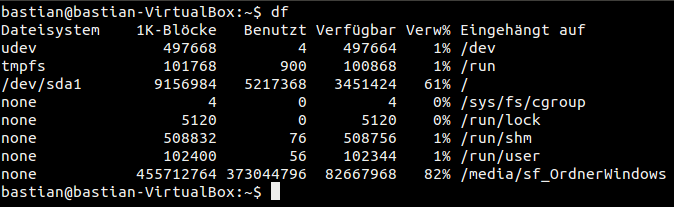
\includegraphics[width=.8\textwidth]{pictures/Bastian/BILD1_df}
\caption{Vorhandene Dateisysteme}
\end{figure}

\subsubsection*{Schritt 2:}
Terminalaufruf für den Backupprozess
\lstset{language=bash,numbers=none,frame=single}
\begin{lstlisting}
sudo dd if=INPUTPARTITION of=OUTPUTFILE
\end{lstlisting}
\begin{tabular}{l c l}
sudo	& -> & Backupprozess benötigt root-Rechte\\
dd	& -> & bit-genaues Kopieren der Dateien\\
if=FILE	& -> & Die Datei oder Partition welche integriert wird\\
of=FILE & -> & Die Output Datei welche angelegt wird\\
\end{tabular}
\newpage %==============================================

\subsubsection*{Schritt 3:}
Optionale Nutzung von Terminalaufruf 'pv' um den Fortschritt des Backup Prozesses zu sehen Die mögliche Restzeit lässt sich nur durch das Hinterlegen der Größe der Partition anzeigen.
\begin{lstlisting}
sudo dd if=INPUTPARTITION |pv| sudo dd of=OUTPUTFILE
\end{lstlisting}
\begin{figure}[ht]
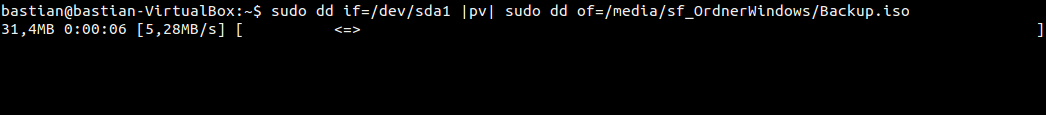
\includegraphics[width=\textwidth]{pictures/Bastian/BILD2_pv}
\caption{Laufender Backupprozess mit Statusanzeige}
\end{figure}
\subsubsection*{Schritt 4:}
Wiederherstellen eines hinterlegten Backups läuft ähnlich wie der ursprüngliche Prozess ab.
\begin{lstlisting}
sudo dd if=OUTPUTFILE |pv| of=INPUTPARTITION
\end{lstlisting}
\begin{figure}[ht]
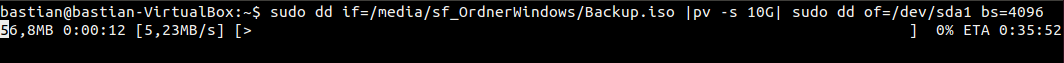
\includegraphics[width=\textwidth]{pictures/Bastian/BILD3_pv}
\caption{Laufender Wiederherstellungsprozess mit Statusanzeige}
\end{figure}
Quelle: https://wiki.ubuntuusers.de/dd/ \cite{dd}
\newpage %==============================================

\subsection{rsync}
Da der Vorgang mittels 'dd' als suboptimal angesehen wird, wurde alternativ der Aufruf 'rsync' verwendet. Dieser bietet die Möglichkeit eines inkrementellen Backups wodurch die Dauer des Prozesses erheblich reduziert werden kann. Hierbei werden die Größe und die Änderungszeit der Dateien in Quelle und Ziel miteinander verglichen. Eine Aktualisierung findet demnach nur statt, wenn Unterschiede vorzufinden sind.
\begin{lstlisting}
rsync -aAXv --delete --exclude={"/dev/*","/proc/*","/sys/*","/tmp/*","/run/*","/mnt/*","/media/*","/lost+found"} / /path/to/backup/folder
\end{lstlisting}
\begin{tabular}{l c l}
rsync	&->& Kopieren der Dateien\\
-aAX	&->& Übertragung im Archiv Modus wodurch alle symbolischen Verweise\\
	&  & beibehalten werden\\
--delete&->& Dateien die im Ursprungsverzeichnis nicht mehr existieren werden\\
	&  & im Zielverzeichnis ebenfalls gelöscht\\
--exclude&->& Dateien werden ausgelassen\\
\end{tabular}\\\\
Wiederherstellen des Rsync Backups durch folgenden Befehl:
\begin{lstlisting}
rsync -aAXv /path/to/backup/location/* /mount/point/of/new/install/ --exclude={/dev/*,/proc/*,/sys/*,/tmp/*,/run/*,/mnt/*,/media/*,/lost+found,/home/*}
\end{lstlisting}
Quelle: https://wiki.ubuntuusers.de/rsync/ \cite{rsync}
\subsection{tar} %===============================================================================
Eine weitere Anwendungsmöglichkeit bietet die 'tar' Archivierung. Vorteil dieses Aufrufs ist, dass durch Angabe von Parametern die Berechtigungen aller zu sichernden Daten ebenfalls beibehalten werden und die Archivierung Speicherplatz spart.\\
Wechsel in das Backupverzeichnis dann:
\begin{lstlisting}
tar -cpzf Backup.tar ORDNER
\end{lstlisting}
\begin{tabular}{l l}
tar	&-> Archivieren von Daten\\
-c	&-> Archiv wird erzeugt (create)\\
-p	&-> Berechtigungen beibehalten (privilige)\\
-z	&-> Zusätzliche Komprimierung mit gzip\\
-f	&-> Archiv in Datei schreiben (finish)\\
\end{tabular}
 ~\\Quelle: https://wiki.ubuntuusers.de/tar/ \cite{tar}

\newpage %==============================================

\subsection{Automatisierung mittels Bash-Skript} %===============================================
Damit der Nutzer die Aufrufe nicht händisch zu bestimmten Zeiten ausführen muss, wurden zwei Bash-Skripte zur Automatisierung geschrieben. Es gibt ein monatliches Backup mittels (tar) und wöchentliche inkrementelle Backups (rsync) auf die zurückgegangen werden kann.\\
\\
Um das Zeitintervall der Backups einzustellen wird der 'Cron' Dienst verwendet.
Hiermit können Skripte und Programme zu festgelegten Zeiten gestartet werden.
Wenn ein hinterlegter Job täglich zu einer bestimmten Uhrzeit ausgeführt wird muss allerdings auch der Rechner zu dem Zeitpunkt aktiv sein. Ist dies nicht der Fall, startet der Prozess nicht. Um dies zu umgehen wird 'Anacron' verwendet.
Durch ablegen des Skripts in eines der entsprechenden Verzeichnisse wird der Prozess entsprechend ausgeführt.\\
Quelle: https://wiki.ubuntuusers.de/Cron/ \cite{cron} \\
\begin{tabular}{l l}
/etc/cron.hourly/	&- Stündlich ausführen\\
/etc/cron.daily/	&- Täglich ausführen\\
/etc/cron.weekly/	&- Wöchentlich ausführen\\
/etc/cron.monthly/	&- Monatlich ausführen\\
\end{tabular}
\begin{figure}[ht]
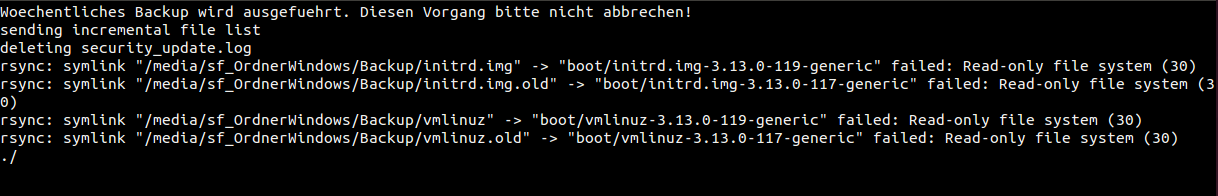
\includegraphics[width=\textwidth]{pictures/Bastian/Woechentliches_Backup}
\caption{Ausführung wöchentliches Backup}
\end{figure}

\section{Update des Banana Pi}
Ziel war es das Betriebssystem und alle Programme immer auf dem aktuellsten Stand zu halten. Hierbei kann es jedoch zu Inkompatibilität bestimmter Funktionen  oder Konfigurationen kommen. Daher wurde die Umsetzung auf die relevantesten Updates (Sicherheitsupdates) reduziert. Im Normalfall können mittels des Konsolenaufrufs  'apt-get update' die Updateliste und mit 'apt-get upgrade' die Programm Pakete selbst aktualisiert werden. Durch Nutzung des Aufrufs 'unattended-upgrade' wird auf Sicherheitsupdates des Systems überprüft und diese anschließend installiert.\\
\\
Durch 'unattended-upgrade --dry-run -d' wird auf Verfügbarkeit von Updates geprüft ohne anschließende Installation. Nach jedem Durchgang wird eine Logdatei in /var/log/unattended-upgrades/ angelegt welche genauere Informationen zu den aktualisierten Dateien liefert.

\section{Implementierung einer Displaystatusanzeige}
Zur besseren Übersicht des Netzwerktraffics als auch der Ressourcen des Banana Pi sollte eine Displaystatusanzeige implementiert werden. Der Aufruf 'htop' bietet eine Übersicht aller laufenden Prozesse und deren Ressourcennutzung. 'iftop' zeigt die Netzwerkinterfaces und die eingehende und ausgehende Kommunikationen. Da das Terminal jedoch nur einen der Befehle zu einem Zeitpunkt ausüben kann wird ein Terminal-Multiplexer verwendet. Zur Auswahl stehen hierbei 'Terminator', 'screen', und 'Tmux'. Aufgrund der geringen Einarbeitungszeit und einfachen Anwendbarkeit wurde letzteres zur Implementation ausgewählt. Alle Multiplexer bieten die Möglichkeit Sitzungen zu erstellen. Leider kann dies nicht zur Implementierung der Displaystatusanzeige verwendet werden, da die Sitzung beim Herunterfahren des Betriebssystems gelöscht wird. Daher wird zum Systemstart ein Bash-Skript eingesetzt, welches automatisch die benötigten Fenster zur Überwachung anlegt.
\begin{figure}[ht]
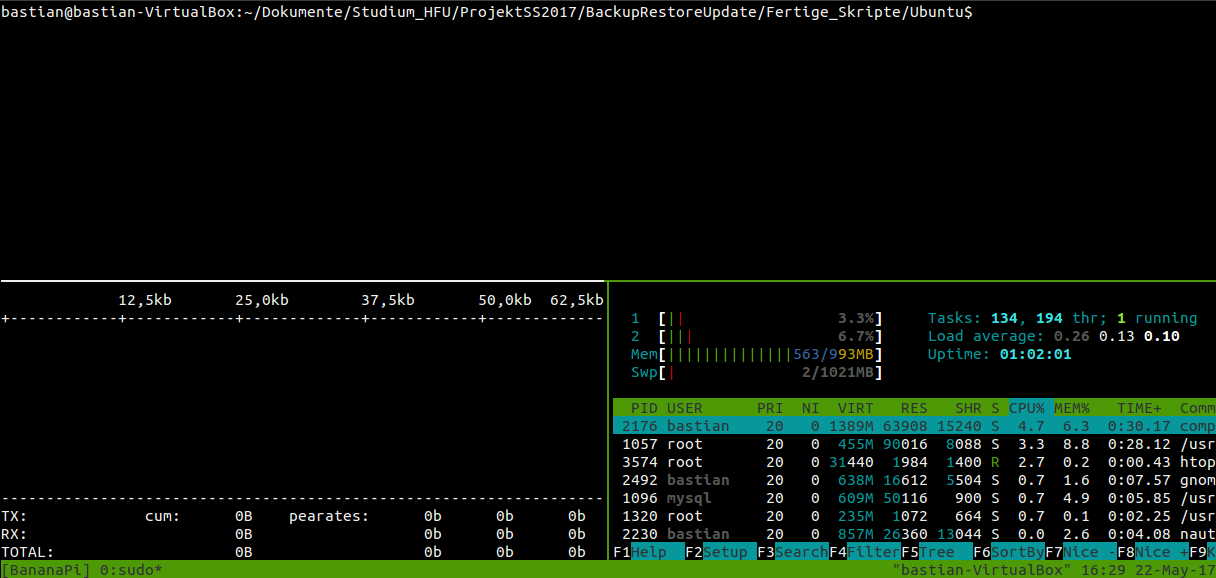
\includegraphics[width=\textwidth]{pictures/Bastian/Tmux}
\caption{Verwendung von Tmux mit 'htop' und 'iftop'}
\end{figure}


\section{Routing, VLANs}

\section{WLAN}

\section{Radius}

\section{Mailserver}

\section{Samba}


\chapter{Benutzeranleitung}

\chapter{Projektbewertung}
Die technischen Herausforderungen des Projekts waren für alle Teilnehmer eine spannende und lehrreiche Erfahrung. Durch die Umsetzung der verschiedenen Implementationsziele auf der gegebenen eingebetteten Plattform können alle Projektteilnehmer einen großen Zugewinn an fachspezifischen Wissen verzeichnen.\\
Mit den wöchentlichen Projekttreffen war es möglich, frühzeitig auf aktuelle Probleme zu reagieren und Lösungsansätze gemeinsam zu erörtern.\\
Aufgrund des Wechsels von Bananian auf Armbian wurde der Zeitplan des Projekts  teils weit zurückgeworfen. Weniger vorweisbare Projekt-Ergebnisse und kleinere Entwicklungsschritte waren die Folge, da Kernfunktionen wie die Switcharchitektur des Banana Pi komplett neu entwickelt werden mussten. Zudem wirkten sich Updates des Betriebssystems teils deutlich auf die Verlässlichkeit und Bedienbarkeit des Geräts aus, was mutmaßlich dem noch unausgereiften Betriebssystem geschuldet ist, das sich zum Zeitpunkt des Projekts in einer sehr aktiven Entwicklungsphase befindet.\\

\chapter{Ausblick}



% Schalgwortverzeichnis (Index)
%\printindex

% Literaturverzeichnis
\singlespacing
\bibliographystyle{plain}
\bibliography{bibtex}

% Eidesstattliche Erklärung
\chapter*{Eidesstattliche Erklärung\markboth{Eidesstattliche Erklärung}{}}
% Eintrag in das Inhaltsverzeichnis 
\addcontentsline{toc}{chapter}{Eidesstattliche Erklärung}

Ich versichere, dass ich die vorstehende Arbeit selbständig verfasst und hierzu
keine anderen als die angegebenen Hilfsmittel verwendet habe. Alle Stellen der Arbeit die 
wörtlich oder sinngemäß aus fremden Quellen entnommen wurden, sind als solche kenntlich gemacht.
\\
\\
Die Arbeit wurde bisher in gleicher oder ähnlicher Form in keinem anderen
Studiengang als Prüfungsleistung vorgelegt oder an anderer Stelle
veröffentlicht.
\\
\\
Ich bin mir bewusst, dass eine falsche Erklärung rechtliche Folgen haben kann.

\vspace*{1.5cm} \par
\line(1,0){200} \par
\docOrt, den  \docAbgabedatum


\appendix
% Hier können Anhaenge angefuegt werden

\end{document}      
